% !TEX program = xelatex
% Clean CV template — Letter (8.5×11in) — requires XeLaTeX
% -------------------------------------------------------------
\documentclass[10pt,letterpaper]{article}

% ---------- FONTS ---------------------------------------------
\usepackage{fontspec}
\IfFontExistsTF{Roboto}
    {\setmainfont{Roboto}}
    {\IfFontExistsTF{Helvetica Neue}
        {\setmainfont{Helvetica Neue}}
        {\setmainfont{Latin Modern Sans}}}

% ---------- GEOMETRY ------------------------------------------
\usepackage[
  letterpaper,
  left=0.55in, right=0.55in,
  top=0.8in,  bottom=0.8in
]{geometry}

% ---------- COLOURS & GRAPHICS --------------------------------
\usepackage[dvipsnames,svgnames,x11names]{xcolor}
\definecolor{primary}{HTML}{004A99}
\definecolor{accent}{HTML}{E6F4FF}

\usepackage{graphicx}
\usepackage{tikz}
\usetikzlibrary{calc}

% ---------- LAYOUT HELPERS ------------------------------------
\usepackage{paracol}
\columnratio{0.32}
\setlength{\columnsep}{0.25in}

\usepackage[most]{tcolorbox}
\tcbset{colback=accent, colframe=accent, boxrule=0pt, sharp corners}

\usepackage{enumitem}
\setlist[itemize]{noitemsep,topsep=0pt,leftmargin=*}

\usepackage{sectsty}
\allsectionsfont{\color{primary}\bfseries\uppercase}
\subsectionfont{\color{primary}\bfseries}
\renewcommand{\thesection}{}

\usepackage{hyperref}

% ---------- UTILITIES -----------------------------------------
\newcommand{\cvName}[1]{\vspace*{0.3in}\textbf{\LARGE #1}}
\newcommand{\cvHeadline}[1]{\par\smallskip\textit{#1}}
\newcommand{\cvHr}{\vspace{0.5\baselineskip}\hrule height 1pt\color{primary}\vspace{0.7\baselineskip}}

% ==============================================================
\begin{document}\small
\begin{paracol}{2}

% ================== SIDEBAR ====================================
\begin{leftcolumn}
\begin{center}
\begin{tikzpicture}
  \node[draw=primary,line width=1pt,circle,minimum width=1.6in]  {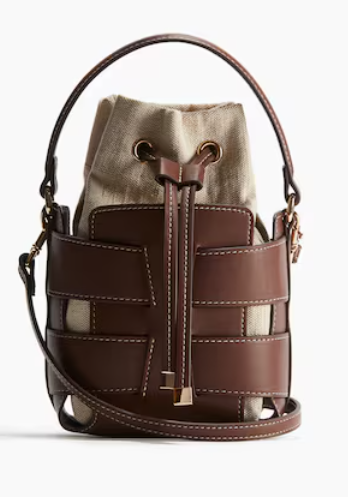
\includegraphics[width=1.45in,height=1.45in,keepaspectratio]{62378246c74040e5820b4f91cadc8e15.png}};
\end{tikzpicture}
\end{center}

\vspace{0.6in}

\cvName{Pape Saliou FALL}
\cvHeadline{Data Scientist}
\cvHr

\section*{Contact}
0753481453\\
\href{mailto:pape@gmail.com}{pape@gmail.com}\\
\url{https://www.linkedin.com/in/pape-saliou-fall-43154a211?lipi=urn%3Ali%3Apage%3Ad\_flagship3\_profile\_view\_base\_contact\_details%3BA855BH4YS42r%2BJJlQ4nODQ%3D%3D}\\
\\

\cvHr
\section*{Languages}
French\\
English

\cvHr
\section*{Key Skills}
Python\\
R\\
SQL\\
Machine Learning
\end{leftcolumn}

% ================== MAIN COLUMN ================================
\begin{rightcolumn}
\section*{Professional Summary}
Data Scientist with 3+ years of experience in developing machine learning models and data pipelines to drive business insights. Strong background in statistical analysis, Python programming, and cloud technologies. Passionate about turning data into actionable strategies and communicating findings to both technical and non-technical stakeholders.

\vspace{1in}
\section*{Work Experience}

\begin{tcolorbox}
  \begin{minipage}[t]{0.48\linewidth}
    Jan 2022\\
    \textbf{Prepaya} --- Data Scientist\\
    \begin{itemize}
      \item Developed and deployed machine learning models for customer churn prediction, improving retention by 15\%.
      \item Built automated data pipelines using Python and SQL, reducing data processing time by 40\%.
      \item Collaborated with cross-functional teams to translate business requirements into analytical solutions.
      \item Visualised insights through interactive dashboards for senior management.
    \end{itemize}
  \end{minipage}\hfill
  \begin{minipage}[t]{0.48\linewidth}\raggedleft
    Dec 2023
  \end{minipage}
\end{tcolorbox}

\vspace{0.9in}
\section*{Education}
\begin{tcolorbox}[colback=white,boxrule=1pt,colframe=primary]
  Master 2 — Data Science\\
  Sorbonne Université\\
  2012 – 2015
\end{tcolorbox}

\section*{Certifications}
\begin{itemize}
  \item ksLD  — KSLQKBC, Jul 2024
\end{itemize}

\section*{Hobbies}
Machine learning competitions • Football

\end{rightcolumn}
\end{paracol}
\end{document}